% Template file for EC papers prepared for A&A 
% prepared by John Peacock, Peter Schneider, Douglas Scott & Patrick Simon 
%
% You need to copy the latest version of the file euclid.sty 
% and the two files aa.bst and aa.cls from A&A into the same directory 
% as your LATEX source file. These files are available on the 
% same Overleaf site from where you got this template file.  
%
% For producing the referee version of you paper, 
% comment out the first of these line, and uncomment the second line 
%
\documentclass[longauth]{aa}
%\documentclass[longauth,referee]{aa}

\usepackage{graphicx}
\usepackage{natbib}
\usepackage{scalerel}

\usepackage[table]{xcolor}

\bibliographystyle{aa}

%%%%%%%%%%%%%%%%%%%%%%%%%%%%%%%%%%%%%%%%
\usepackage{txfonts}
%%%%%%%%%%%%%%%%%%%%%%%%%%%%%%%%%%%%%%%%
\usepackage[pdfencoding=auto,psdextra]{hyperref}
\hypersetup{
    colorlinks=true,
    linkcolor=blue,
    filecolor=magenta,      
    urlcolor=blue,
    citecolor=blue
}
\urlstyle{tt}

% suppress these aa-package warnings:
% package hyperref warning: suppressing link with empty target
\makeatletter
\renewcommand*\aa@pageof{, page \thepage{} of \pageref*{LastPage}}
\makeatother

% To add links in your PDF file, use the package "hyperref"
% with options according to your LaTeX or PDFLaTeX drivers.
%
\usepackage[utf8]{inputenc}

\usepackage[switch, modulo]{lineno}
              
    % For a version without line numbering, just comment out
    % the following line 
\linenumbers
    %

\usepackage{euclid}


\begin{document}
%
% Put the title and authors of your (Standard Project) paper here
%

\title{\Euclid\/: Deep-learning super-resolution of NISP imaging and its fidelity for galaxy shape measurement\thanks{This paper is published on behalf of the Euclid Consortium}}

%% please do not edit the author list once you copy it from the
%% Publication Portal -- contact ECEB Bureau for changes

%% please do not edit the author list -- contact ECEB Bureau for changes
% \newcommand{\orcid}[1]{} %% define as link to https://orcid.org/#1 if needed
% \newcommand{\orcid}[1]{} %% if already defined in aa.cls: comment, or use renewcommand			   

\author{\normalsize E.~Everetts$^{1,2}$\thanks{\email{eaev@ipac.caltech.edu}}, S.~Hemmati$^{1}$, K.~Finner$^{1}$, A.~Haghjoo$^{3}$, E. ~Huff$^{4}$, D.~Scognamiglio$^{4}$, et al.}

\institute{$^{1}$ Caltech/IPAC, Pasadena, CA, USA\\
$^{2}$ University of California, Berkeley, Berkeley, CA, USA\\
$^{3}$ University of California, Riverside, Riverside, CA, USA\\
$^{4}$ NASA/JPL, Pasadena, CA, USA\\}
%%%% please do not edit the author list -- contact ECEB Bureau for changes

   
%
% For a Key Project paper, please use instead:
%
% \title{\Euclid\/ preparation} % or another appropriate pre-phrase
% \subtitle{Your title}
%
% \author{Euclid Collaboration: F.~Author, .....}
%

% \institute{$^{1}$ Dark Energy Institute\\
% $^{2}$ Center for Large-Scale Structure\\
% $^{3}$ Institute for Fundamental Research \\
% $^{4}$ Institute for Astrophysics and Cosmology\\}

% 
% Put your abstract here:
%
\abstract{
\Euclid's near-infrared NISP imaging offers access to galaxy populations relevant to weak lensing, but its coarse sampling limits measurements of galaxy structure.
We investigate whether learned super-resolution improves image fidelity and observed shapes while preserving sensitivity to applied shear.
We train a conditional diffusion model and two residual-network variants on 17\,816 NISP \YE-band cutouts paired with JWST/NIRCam F115W images, and evaluate them on 2118 validation galaxies.
Residual networks achieve lower reconstruction errors and stronger spatial correlation with JWST than diffusion, whereas diffusion retains more observed small-scale power.
Relative to native NISP, ResNet reduces ellipticity-component RMSE by approximately 19\% with fixed weighted moments and 11\% with adaptive moments on matched successful samples.
Improvements are largest at high signal-to-noise; low-signal comparisons are limited by measurement selection.
Reconstruction errors are consistent across three training seeds.
Controlled simulations using supplied NISP effective point-spread functions show increased ResNet shear response for compact galaxies, but gains depend on size and noise, and responses remain below intrinsic values.
These results support residual networks as a promising approach to improving observed-shape fidelity in NISP imaging and motivate further investigation for weak lensing.
Establishing calibrated shear accuracy will require realistic simulations and independent validation that account for noise, instrumental response, cross-band differences, and measurement selection.
}

%
% Provide up to five key words:
%
    \keywords{Gravitational lensing: weak -- Methods: data analysis -- Techniques: image processing -- Surveys}
%    from the list in
%     https://www.aanda.org/for-authors/latex-issues/information-files#pop}
%
% Add short versions of title and author list for page headings
%
   \titlerunning{\Euclid\/: Super-resolution of NISP imaging and its fidelity for shape measurement}
   \authorrunning{E.~Everetts et al.}
   
   \maketitle
%
%-------------------------------------------------------------------
%
%
%   Start the main text of your paper here
%
   
\section{Introduction}
\label{sc:intro}

Weak gravitational lensing is one of the primary cosmological probes of
Stage IV wide-field surveys \citep{Laureijs2011, Chang2013}, and its
statistical precision places increasingly demanding requirements on the
control of systematic errors. Shape measurement in particular has required a sustained,
community-wide effort to characterize and control: successive blind
challenges \citep{Heymans2006, Massey2007, Mandelbaum2015} and
dedicated calibration frameworks based on image simulations and
self-calibration \citep[e.g.,][]{Huff2017, Sheldon2017,
EC_Congedo2024} have been devoted to measuring and removing biases in
classical shape estimators at the level modern surveys require. For
\Euclid, multiplicative shear biases must be controlled to
$\sim$$10^{-3}$ \citep{Cropper2013}. New shape-measurement techniques must therefore be tested for biases
and calibrated before their outputs can support cosmological inference.

Deep learning has meanwhile become integral to astronomical data
analysis, with applications ranging from image generation and outlier
detection to photometric redshift estimation and deblending in crowded
fields \citep{Arcelin2021, Hemmati2022, Sampson2024, Scognamiglio2025}.
Among these, super-resolution, the task of inferring high-resolution
spatial information from lower-resolution inputs \citep{Anwar2019}, has
been applied across regimes from radio interferometry to solar and
ground-based optical imaging \citep[e.g.,][]{Dabbech_2022, Song2024,
Sukurdeep2025}. In \Euclid, weak-lensing shapes are measured in the
visible band with VIS \citep[$0\farcs1$ pixels;][]{EuclidSkyVIS}, while
the near-infrared imaging from NISP
\citep[$0\farcs3$ pixels;][]{EuclidSkyNISP} is coarser by a factor of
three in sampling and is not used for shape measurement. As a result, a
population of galaxies that is well detected in the near-infrared,
including red and high-redshift sources for which VIS shapes are
unavailable, is excluded from the weak-lensing sample.
Studies using HST/CANDELS imaging have demonstrated the potential of
near-infrared shapes: \citet{Lee2018} compared ellipticity measurements
in optical and near-infrared images degraded to survey quality, while
\citet{Finner2023} examined WFC3-IR PSF modelling and weak-lensing systematics.
Super-resolved NISP images could extend the range of galaxies with
useful shape measurements, increasing the source density and redshift
coverage available to lensing analyses. Assessing this possibility
requires both a comparison with higher-resolution observations and a
test of whether the reconstructed shapes remain sensitive to applied shear.

We train deep-learning super-resolution models on \Euclid\ NISP images
of the COSMOS field and evaluate them against overlapping JWST/NIRCam
imaging of the same region, which provides a factor of five finer pixel
sampling and an independent, higher-resolution reference for every
galaxy in the sample (Sect.~\ref{sc:observations}).
A conditional diffusion model \citep{sohldickstein2015, Ho2020} generates
images through successive denoising steps, while a residual network
built from residual dense blocks \citep{Wang2018} predicts an image in
a single pass. Both learn from the paired training data and therefore
combine information in the NISP image with patterns learned from the
training population. Their different objectives and reconstruction
procedures allow us to test the trade-off between image error, spatial
structure, and shape fidelity (Sect.~\ref{sc:methods}).

We evaluate the models on regional image fidelity, spatial structure, and observed ellipticity measured with fixed and adaptive moments (Sect.~\ref{sc:results}).
The residual models reduce image and shape errors against the observed JWST reference, while diffusion retains more small-scale power.
We examine how shape errors and measurement coverage vary with input signal-to-noise, and separately test the original ResNet's response to applied shear in controlled simulations using the supplied NISP effective PSFs.
The latter experiment measures sensitivity to a known distortion; the cross-band ellipticity-fit slopes are not shear-calibration factors.
These comparisons identify benefits and remaining limitations of the selected models, while applications to morphology, deblending, or lens identification require validation for each task (Sect.~\ref{sc:discussion}).

%\cite{EuclidSkyOverview}

\section{\label{sc:observations}Observations}

We use \Euclid\ NISP \YE-band imaging \citep{EuclidSkyNISP} and overlapping JWST/NIRCam F115W imaging \citep{jwst_nircam} in the COSMOS field \citep{Scoville_2007}.
The NISP images are co-added products from the \Euclid\ Quick Release Q1 \citep{Q1cite}, processed by the NIR pipeline at approximately $0\farcs3$ per pixel \citep{Q1-TP003}.
The JWST images come from COSMOS-Web \citep{cosmos_web_overview}; we use its F115W mosaics at $0\farcs06$ per pixel, compared with the detector's approximately $0\farcs03$ sampling.
The \YE\ and F115W passbands overlap but are not identical, so differences in the spatial distribution of stellar populations and dust can contribute to differences between the images.

The output grid samples the sky five times more finely than the NISP input.
This change in sampling does not specify the improvement in recovered resolution: the target images retain the JWST point-spread function (PSF), mosaic resampling, and the additional interpolation described in Sect.~\ref{sc:preprocessing}.
We therefore evaluate the reconstructions against the observed F115W images without assigning them a deconvolved PSF.
We extract $41\times41$ NISP cutouts and construct $205\times205$ target images over the same approximately $12\arcsec$ field, providing room around each galaxy for background and neighbour measurements.

We select COSMOS2020 Classic galaxy-class objects (\texttt{lp\_type}$=0$) with ACS F814W AB magnitude $<25$, EAZY photometric redshift $0.01<z_{\rm phot}<3$, and $4<\texttt{FLUX\_RADIUS}<500$ in catalog pixels.
The catalog radius encloses half of the flux in the PSF-homogenized $K_s$ image; it is not a radius measured in JWST pixels \citep{cosmos2020_classic}.
The optical magnitude threshold is motivated by the approximate $riz<25$ Euclid-depth selection adopted by \citet[Section~5.2]{shooby_calibration}, with F814W serving here as an optical-band proxy rather than an equivalent Euclid passband.
Their WFIRST lensing-analog selection also illustrates the joint role of brightness and angular size in obtaining measurable galaxy shapes \citep[Section~2.3 and Figure~3]{shooby_calibration}.
Our catalog cuts define the sample for resolved-morphology analysis; they do not implement that survey-specific shape-quality selection or establish a NISP detection limit.

The input inventory contains four NISP \YE-band stacks and 19 F115W mosaics; the accepted galaxy pairs draw on all four stacks and 18 of the JWST mosaics.
Each JWST mosaic spans $9600\times12455$ pixels, or approximately $9\farcm6\times12\farcm5$ at the adopted sampling, with usable coverage determined by the validity masks.
Starting from 39\,024 coverage candidates identified using the COSMOS2020 Classic catalog \citep{cosmos2020_classic}, the extraction retains 22\,810 paired galaxies after coverage, pixel-quality, and spatial-buffer cuts.
We assign disjoint $3\arcmin$ sky blocks to training, validation, and test subsets, excluding galaxy centres within $10\arcsec$ of block boundaries.
The resulting samples contain 17\,816 training, 2\,118 validation, and 2\,876 test galaxies.
Training data are used to fit model weights and normalization scales; validation data support checkpoint selection and model and measurement-protocol development.
All comparisons of observed galaxies use the validation sample; the test sample remains unused and is reserved for an independent evaluation of the final model and measurement protocol.
This spatial separation reduces overlap between neighbouring cutouts across splits, although all three subsets sample the same COSMOS field.
Figure~\ref{fig:sample_overview} shows the spatial distribution and an illustrative pair of observed images.
Figure~\ref{fig:sample_properties} compares the magnitude and redshift distributions of the three subsets with the full COSMOS2020 parent catalog selected only by valid ACS F814W magnitude $<25$, with no other population cuts.

\begin{figure*}[t]
    \centering
    % Frozen export from paper_figures/01_sample.ipynb, version v08.
    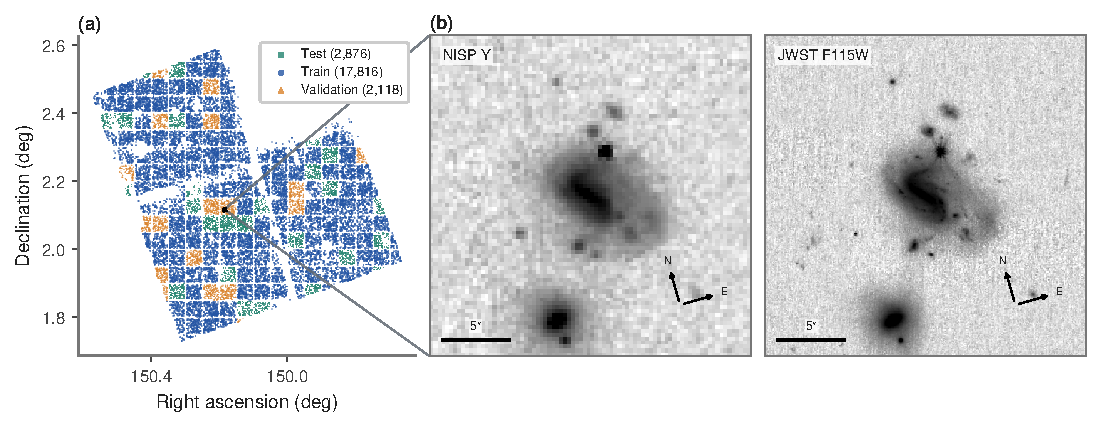
\includegraphics[width=\textwidth]{figs/sample_overview_v08.pdf}
    \caption{Matched \Euclid\ NISP and JWST sample in COSMOS.
    (a) Galaxy positions in the training (cobalt circles), validation (orange triangles), and test (green squares) subsets, defined by $3\arcmin$ sky blocks with $10\arcsec$ boundary buffers.
    (b) NISP \YE-band and JWST/NIRCam F115W views of a $24\farcs3\times24\farcs3$ field around an example galaxy, marked in (a).
    Both images use the same surface-brightness stretch. Scale bars indicate $5\arcsec$; arrows show north and east.}
    \label{fig:sample_overview}
\end{figure*}

\begin{figure*}[t]
    \centering
    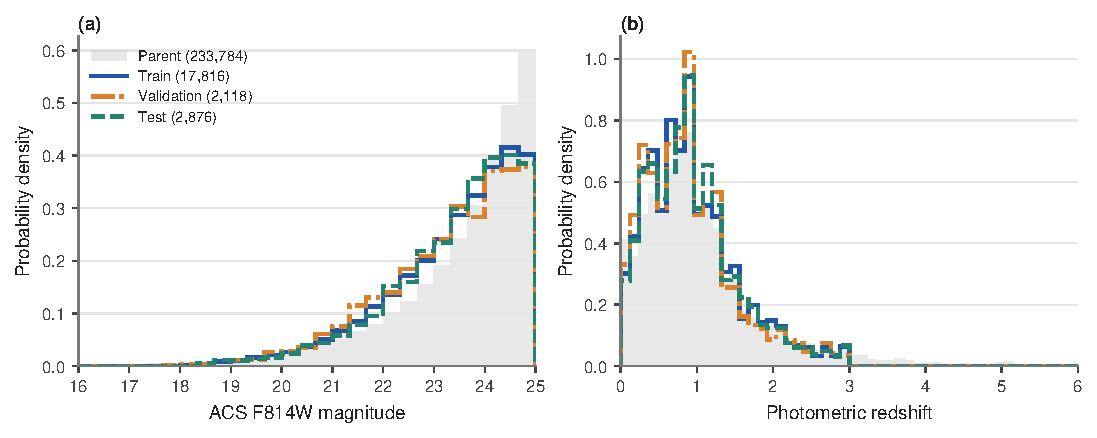
\includegraphics[width=\textwidth]{figs/sample_properties_v06.pdf}
    \caption{ACS F814W magnitude (a) and photometric-redshift (b) distributions of the training (solid cobalt), validation (dash-dotted orange), and test (dashed green) samples.
    Gray shading shows the full COSMOS2020 catalog with only valid ACS F814W magnitude $<25$; no classification, footprint, redshift, size, or quality cuts are applied to the parent. Invalid redshifts are omitted only from the redshift histogram.
    Histograms use common bins and are normalized by all valid measurements in each sample, including those outside the displayed ranges.}
    \label{fig:sample_properties}
\end{figure*}

\section{\label{sc:methods}Methods}

We compare a conditional diffusion model and two variants of a residual convolutional network for reconstructing JWST F115W images from NISP \YE-band observations.
The diffusion model generates an image through repeated updates starting from random noise; the residual networks predict an image in a single pass.
All models learn from the paired training images, so their reconstructions depend on both the NISP measurements and the galaxy population represented in the training sample.
Our main objective is recovery of the \emph{observed} F115W galaxy shapes, alongside image fidelity.
The reference images retain the JWST point-spread function (PSF), instrumental noise, and the effects of resampling; agreement with them does not by itself establish accurate intrinsic shapes or calibrated gravitational shear.

\begin{figure*}
    \centering
    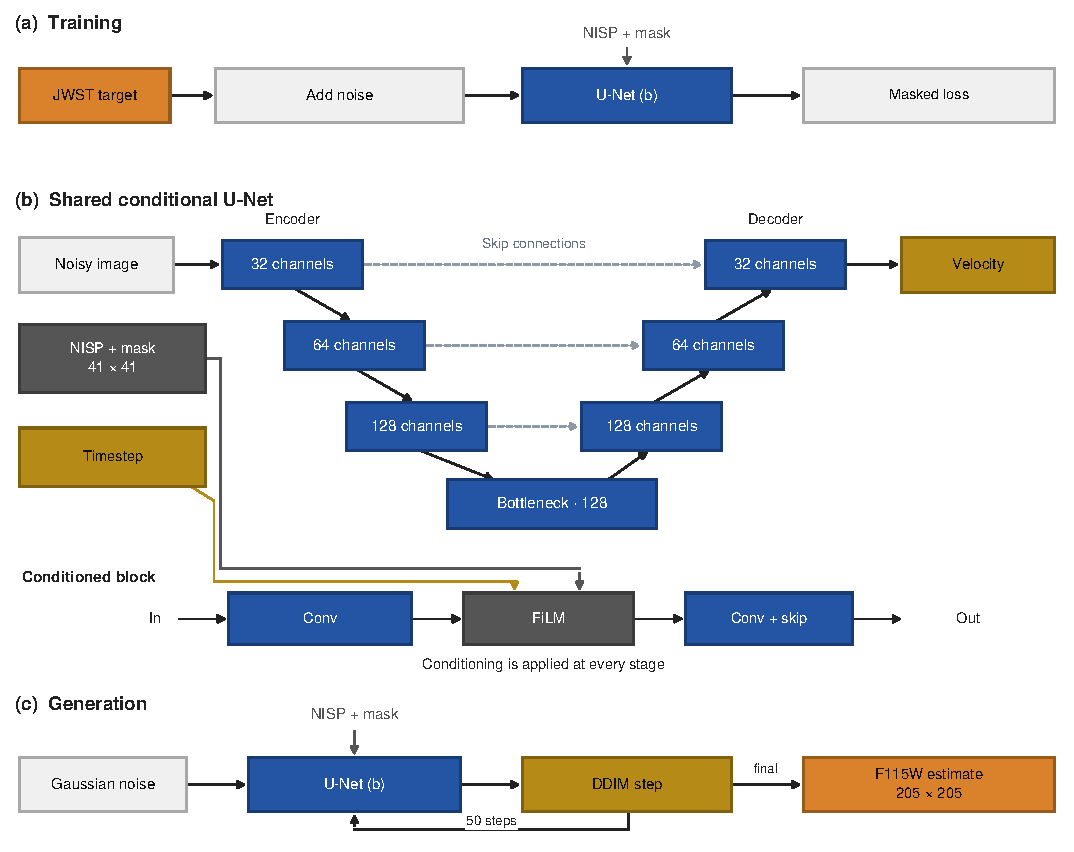
\includegraphics[width=\textwidth]{figs/diffusion_architecture_v06.pdf}
    \caption{Diffusion model for reconstructing F115W images from NISP observations.
    (a) Training uses JWST targets with added noise; errors are measured only over valid target pixels.
    (b) The U-Net combines image features at several spatial scales, with the number of feature maps indicated in each stage. The NISP image, its validity mask, and the noise level guide the updates within each block through learned rescalings and offsets (FiLM).
    (c) Starting from Gaussian noise, 50 successive updates produce a $205\times205$ F115W estimate. The prediction is converted back to surface brightness before evaluation.}
    \label{fig:diff_model}
\end{figure*}

\subsection{Image preparation}
\label{sc:preprocessing}

We construct paired cutouts using the COSMOS2020 coordinates and the world coordinate system (WCS) of each mosaic.
The NISP cutout contains $41\times41$ native pixels and is extracted with \texttt{Astropy}'s \texttt{Cutout2D} \citep{astropy_latest}, without rotating or interpolating its pixel values.
We define a $205\times205$ output grid with the same sky footprint and orientation, subdividing each NISP pixel into $5\times5$ target pixels.
The resulting sampling is approximately $0\farcs06$ per target pixel over a $12\farcs3$ field.
Each target pixel is mapped through the two WCS solutions to the JWST mosaic, where its surface brightness is obtained by bilinear interpolation using \texttt{SciPy} \citep{scipy}.
This mapping accounts for the relative orientation, pixel scale, and position of the mosaics in one resampling step.
We apply no additional shifts fitted from the galaxy images; residual errors in the survey astrometry can therefore contribute to reconstruction differences.

The two instruments retain separate validity masks.
A NISP pixel is valid when its science value is finite, its data-quality flag is zero, and its supplied root-mean-square (RMS) uncertainty is finite, positive, and below the mosaic's large invalid-value range ($10^7$ in the native units).
For the available JWST science mosaics, which lack accompanying quality and uncertainty maps in this dataset, we use finite, nonzero pixels as a coverage proxy.
An interpolated target pixel is valid only when all contributing source pixels are valid.
We require at least 95\% valid pixels in each cutout and complete coverage of the central $5\times5$ NISP pixels and corresponding $25\times25$ target pixels.
These requirements supplement the catalog and spatial selections in Sect.~\ref{sc:observations}; the JWST coverage proxy does not replace a full data-quality assessment.

We estimate and subtract a constant background separately for each image using the median of valid outer pixels after $3\sigma$ clipping, with at most five iterations.
The central square, approximately half the cutout width, is excluded from this estimate.
NISP fluxes in $\mu$Jy per pixel are converted to MJy\,sr$^{-1}$ using the local pixel solid angle from the WCS; JWST images are already in MJy\,sr$^{-1}$.
For numerical stability, each band is divided by a fixed scale determined from the training set alone.
The NISP scale is the median, across training cutouts, of the median supplied pixel RMS in surface-brightness units; the JWST scale is the median clipped outer-region standard deviation.
The resulting scales are 0.02307 and 0.01365\,MJy\,sr$^{-1}$ for NISP and JWST, respectively.
They are held fixed for validation and test data; individual galaxies are not normalized by their own flux or target variance.

Invalid pixels are filled with zero after background subtraction and scaling, and valid negative intensities are retained.
The residual networks use these linearly scaled images; the diffusion model uses the additional reversible transformation described below.
All physical image and shape comparisons use background-subtracted linear intensities, with the transformations inverted and no clipping of negative values.
Training losses exclude invalid target pixels and give each galaxy equal weight.
No PSF deconvolution or filter-response correction is applied.
The learned mapping therefore includes the difference between the \YE\ and F115W bands and their instrumental responses; we do not assume that a reconstructed image has a known effective PSF.
Bilinear resampling also changes the target PSF and noise correlations, which are not explicitly modeled here.

\subsection{Diffusion model architecture}
\label{sc:diffusion_model}

Our diffusion model builds an estimate of the JWST F115W image through a sequence of small updates, guided throughout by the observed NISP image.
It follows the image-refinement approach of \citet{SR3}, based on denoising diffusion models \citep{Ho2020, Nichol2021}.
During training, we add a known amount of Gaussian noise to a JWST cutout and teach the network to recover information about the original image.
Repeating this task at different noise levels teaches the model how to proceed from an initially random image towards an F115W reconstruction.
Figure~\ref{fig:diff_model} shows the training procedure, network structure, and generation of a new image.

The NISP input contains $41\times41$ pixels, and the F115W output contains $205\times205$ pixels over the same sky area.
We use bilinear interpolation to place the NISP image on the output grid as a spatially aligned guide.
A second input map identifies valid NISP pixels, allowing the network to distinguish missing data from measured low surface brightness.
Missing input values are set to zero; the validity map is resized using nearest-neighbour interpolation.
Before entering the network, both bands are passed through the inverse hyperbolic sine transformation, $\mathrm{asinh}(I/3)$, where $I$ is the background-subtracted intensity divided by its training-set scale (Sect.~\ref{sc:preprocessing}).
This reversible transformation compresses the range of bright intensities while retaining negative values from background subtraction.
The intensity transformation is applied before resizing the NISP conditioning image and is reversed before physical evaluation.

The network has a U-Net structure: an encoder successively reduces the spatial resolution to describe broader image structure, and a decoder restores the resolution to produce the output.
The encoder levels contain 32, 64, and 128 feature maps, or \emph{channels}; a central stage retains 128 channels, and the decoder returns through the same levels in reverse order.
Connections between corresponding encoder and decoder levels pass their feature maps directly to the reconstruction path, helping to retain spatial information.
Each stage contains two residual blocks, which learn corrections that are added to the features entering the block.
The NISP image and its validity map provide guidance at every stage; the current noise level is also supplied to the network.
These inputs control learned rescalings and offsets of the internal features, a procedure called feature-wise linear modulation (FiLM; \citealt{Perez2017}).
The network temporarily pads the images from 205 to 208 pixels on a side to accommodate its changes in resolution, then crops the output back to the target grid.

For each training pair, we uniformly sample one of 1000 noise levels from a cosine schedule, with the final level containing only Gaussian noise.
Writing the transformed target as $x_0$ and a standard Gaussian noise field as $\epsilon$, the noisy image and the quantity predicted by the network are
\begin{equation}
    x_t=a_t x_0+b_t\epsilon, \qquad v_t=a_t\epsilon-b_t x_0,
\end{equation}
where $a_t=\sqrt{\bar\alpha_t}$, $b_t=\sqrt{1-\bar\alpha_t}$, and $\bar\alpha_t$ is the fraction of signal variance retained at step $t$.
The quantity $v_t$, labelled \emph{velocity} in Fig.~\ref{fig:diff_model}, is thus a noise-dependent combination of the original image and the added noise.
From the network prediction $\hat v_t$, the reconstructed target is $\hat x_0=a_t x_t-b_t\hat v_t$, which remains defined even at the pure-noise endpoint.
We minimize
\begin{equation}
    \mathcal{L}_{\rm diff}
    =\left\langle(\hat v_t-v_t)^2\right\rangle_V
    +0.1\left\langle|\hat x_0-x_0|\right\rangle_V,
\end{equation}
where $\langle\cdot\rangle_V$ denotes an average over valid JWST pixels within each galaxy, followed by an average over galaxies in the batch.
Both terms are evaluated in the transformed intensity coordinates.

To generate an image, we start from a random Gaussian field on the output grid and repeatedly apply the trained network using the NISP image and its validity map as guidance.
The JWST target is used only for training and evaluation.
We use 50 updates with the denoising diffusion implicit model (DDIM) procedure of \citet{Song2021DDIM}, which allows generation with fewer steps than the number of noise levels used during training.
No further random noise is added during these updates, so a fixed initial noise field gives a reproducible reconstruction.
Changing that initial field produces different reconstructions for the same NISP input.
We retain the full range of predicted intensities and convert the final image back to linear surface brightness.

\subsection{Residual network architecture}
\label{sc:residual_model}

The residual network produces an F115W estimate from the NISP image in a single pass.
Its layers first extract features on the original $41\times41$ grid, then enlarge these features and combine them into a $205\times205$ output image.
We compare two variants with the same feature-extraction structure and different enlargement paths: the two-stage residual network (ResNet) and the direct-$5\times$ residual network (ResNet-D5; Fig.~\ref{fig:resnet_model}).
Each variant is trained separately.

\begin{figure*}
    \centering
    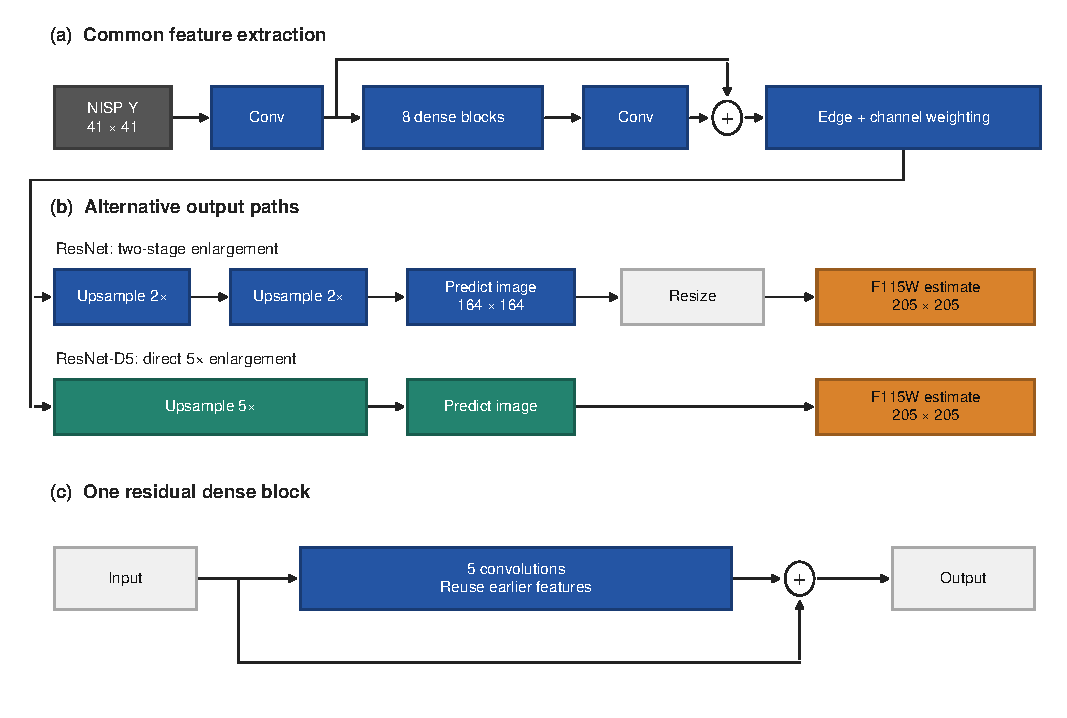
\includegraphics[width=\textwidth]{figs/residual_architecture_v06.pdf}
    \caption{Residual network for reconstructing F115W images from NISP observations.
    (a) Both variants extract features using eight residual dense blocks, followed by edge filtering and learned weighting of the feature maps.
    (b) Two separately trained variants use different enlargement paths. ResNet enlarges twice by $2\times$, predicts an image on a $164\times164$ grid, then resizes it to $205\times205$; ResNet-D5 enlarges directly by $5\times$ and predicts on the target grid.
    (c) Within each dense block, convolutions reuse earlier features and add a learned correction to the input. Plus symbols denote this addition.}
    \label{fig:resnet_model}
\end{figure*}

The feature-extraction part combines residual learning \citep{ResNet} with the reuse of intermediate features found in image super-resolution networks \citep{Wang2018}.
An initial convolution produces 64 feature maps, which pass through eight residual dense blocks.
Within each block, successive convolutions receive the block input together with the features produced by earlier layers.
This reuse of earlier information is what the term \emph{dense} describes.
The first four convolutions each produce 32 additional feature maps; a fifth combines the accumulated information into 64 maps.
The block then adds this learned correction to its input, forming the residual connection.
After all eight blocks, another convolution combines the features, and a longer connection adds back the maps from the initial layer.

An additional module emphasizes spatial changes in these feature maps.
It applies a fixed edge-detection filter to each map, adds the filter response to the original features, and processes the result with learned convolutions.
The network also assigns a weight to each feature map using its average response across the image, following the channel-weighting approach of \citet{hu2019}.
These learned weights adjust the contribution of each map before enlargement.
The module operates on internal features; its effect on the reconstructed galaxy shapes is evaluated with the rest of the network.

The two enlargement paths use \emph{pixel shuffling}: a convolution predicts additional feature maps, whose values are rearranged into neighbouring positions on a finer grid \citep{Shi2016PixelShuffle}.
ResNet doubles the grid size twice, from 41 to 82 and then 164 pixels on a side.
Two final convolutions combine the features into an image, which is resized by bilinear interpolation to the required $205\times205$ grid.
ResNet-D5 enlarges the features in one step from 41 to 205 pixels, then predicts the image on that grid.
This comparison tests whether reconstructing directly at the target sampling improves image and shape recovery.
ResNet-D5 also has more parameters (Table~\ref{tab:training_settings}), so the comparison includes a change in model capacity.

Both variants take the linearly scaled NISP intensity image as their sole network input, with invalid input pixels set to zero as described in Sect.~\ref{sc:preprocessing}.
The output is converted back to surface brightness without clipping its range.
Each model is trained from initialization using the mean absolute difference between its prediction and the JWST target, averaged over valid target pixels within each cutout and then over galaxies.
This objective measures errors in linearly scaled intensity, whereas the diffusion loss operates in the transformed coordinates defined above.

\subsection{Training and model selection}
\label{sc:training}

All three models use the same 17\,816 training galaxies and a budget of 50 epochs, corresponding to 111\,350 optimizer updates at batch size eight.
We apply random multiples of $90\degr$ rotation and reflections consistently to each paired batch, including its masks and noise maps; validation images are not augmented.
Training uses Adam and a learning rate that rises during the first 30\% of updates and then decays with a cosine profile.
The initial, maximum, and final learning rates are $4\times10^{-6}$, $10^{-4}$, and approximately $4\times10^{-10}$, respectively.
Table~\ref{tab:training_settings} summarizes the common settings and the differences between models.
The equal update budget does not imply equal computation: the models differ in parameter count, objective, intensity representation, and image-generation cost.

We select the saved model with the lowest validation mean absolute image error after an epoch.
For the residual networks, this uses all 2118 validation galaxies; the linearly scaled error used during selection differs from the physical error by one fixed multiplicative factor, so both select the same model.
For diffusion, generating a validation sample requires 50 network evaluations per galaxy.
We therefore monitor a fixed, randomly selected subset of 256 validation galaxies, with a fixed initial noise field for each galaxy, and select by mean absolute error in MJy\,sr$^{-1}$.
Generation uses only the NISP input and its mask; the JWST image and mask enter the comparison afterwards.
The evaluation protocol then applies the selected model to the full validation sample.

To assess variation with the initial diffusion noise, the full-validation protocol generates three independently seeded images per galaxy.
We compare their shape errors on the same successful objects and also evaluate the mean of the three images, formed in linear surface brightness before measuring its shape.
The mean image is treated as a separate reconstruction; averaging ellipticities is not equivalent to measuring that image.
Variation among these draws describes sampling variability, rather than a calibrated uncertainty on the true galaxy image.

Shape measurements support validation-stage analysis and method development but do not select the training checkpoints.
The main architecture comparison uses training seed 20261016.
For ResNet, we additionally repeat the complete 50-epoch training with independent seeds 20261018 and 20261019, keeping the data, architecture, normalization, optimization schedule, and checkpoint criterion fixed.
These repetitions assess variation between training runs; they do not replace the original checkpoint with the most favourable seed.
Diffusion and ResNet-D5 retain one training seed each.
The runs use PyTorch 2.6.0 on NVIDIA L40S GPUs, with recorded data, source, and checkpoint hashes.
Losses, validation metrics, and fixed galaxy examples are monitored with Weights \& Biases \citep{wandb}.

We also compare two matched ten-epoch continuations from the original epoch-49 ResNet checkpoint, preserving its optimizer state and using identical batches and augmentations with a cosine learning-rate decay from $10^{-5}$ to $10^{-6}$.
One retains the original valid-pixel mean absolute error; the other gives equal weight to the per-object source and outside-source mean absolute errors, using the detection prescription in Sect.~\ref{sc:regional_structure}.
Both continuations select the lowest source-region validation mean absolute error, including the unchanged parent as a candidate; this differs from the full-field criterion used for the primary comparison.

We further test two PSF-aware continuations that add the input RMS map, validity mask, and an encoding of the associated NISP stack PSF.
A small adapter adds these features after the first convolution; its output is initialized to zero so that the initial prediction matches the original ResNet exactly.
One variant also receives a regularized inverse-filter residual, while retaining the unfiltered NISP image.
For these features, the supplied PSF is centred and resampled onto an $11\times11$ native-grid kernel using its header geometry, then normalized to unit sum.
The inverse filter uses the transfer function $H^*(1+\lambda)/(|H|^2+\lambda)$, where $H$ is the kernel's Fourier transform and $\lambda=0.05$, with reflection padding to limit edge effects.
This is an approximate effective-PSF treatment; it does not define a calibrated deconvolution.

Both variants use the original-loss control's batches, augmentations, objective, and ten-epoch budget, with the same source-MAE checkpoint criterion.
Inherited parameters retain their optimizer state and learning-rate schedule; new adapter parameters use fresh Adam state and a cosine decay from $10^{-4}$ to $10^{-5}$.
The added inputs are transformed consistently with the image during augmentation, and no target-derived information is supplied at inference.
These experiments test whether PSF and noise information improve the existing model beyond additional training alone; their results inform the model choice in Sect.~\ref{sc:resnet_selection}.

\begin{table*}[t]
    \caption{Architecture, training, and generation settings.}
    \label{tab:training_settings}
    \centering
    \begin{tabular}{lccc}
        \hline\hline
        Setting & Diffusion & ResNet & ResNet-D5 \\
        \hline
        Trainable parameters & 4\,910\,593 & 2\,332\,177 & 2\,959\,953 \\
        Feature channels & 32, 64, 128 & 64 & 64 \\
        Residual blocks & 14 & 8 dense & 8 dense \\
        Network conditioning/input & NISP + validity mask & NISP & NISP \\
        Intensity representation & $\mathrm{asinh}(I/3)$ & Linear & Linear \\
        Training objective & $v$ MSE + $0.1x_0$ MAE & Image MAE & Image MAE \\
        Gradient-norm limit & 1 & None & None \\
        Checkpoint-selection galaxies & 256 & 2118 & 2118 \\
        Training noise levels & 1000 (cosine schedule) & --- & --- \\
        Generation & 50 DDIM updates & Single pass & Single pass \\
        \hline
        Training galaxies & \multicolumn{3}{c}{17\,816} \\
        Batch size & \multicolumn{3}{c}{8} \\
        Training budget & \multicolumn{3}{c}{50 epochs; 111\,350 updates} \\
        Optimizer & \multicolumn{3}{c}{Adam; no weight decay} \\
        Learning-rate schedule & \multicolumn{3}{c}{OneCycle; maximum $10^{-4}$; 30\% rise, then decay} \\
        Checkpoint criterion & \multicolumn{3}{c}{Lowest validation mean absolute image error} \\
        Full validation sample & \multicolumn{3}{c}{2118 galaxies} \\
        \hline
    \end{tabular}
    \tablefoot{All losses average valid pixels per galaxy before averaging galaxies.
    $I$ is the background-subtracted intensity divided by the training-set scale.
    The diffusion schedule ends at zero signal; DDIM adds no further noise after initialization.
    The residual two-stage variant uses two $2\times$ pixel-shuffle steps followed by bilinear resizing to the $5\times$ target grid.
    The common budget specifies the training protocol and does not establish convergence.}
\end{table*}

\subsection{Image and observed-shape comparisons}
\label{sc:measurement}

We evaluate image fidelity using the mean absolute error over valid JWST pixels, first within each cutout and then across galaxies, in MJy\,sr$^{-1}$.
The training monitor also records a root mean squared error (RMSE), taking the square root after averaging the per-galaxy mean squared errors.
For the regional image comparison in Fig.~\ref{fig:pixel_comp}, we instead compute RMSE within each galaxy and region before averaging galaxies with equal weight; these two aggregation conventions are distinct.
Training losses from different intensity representations are not compared as physical image errors.
For shapes, we compare reconstructed images with the JWST reference, native NISP images, and bilinear and bicubic enlargements of NISP on the common target grid.
Interpolation uses the background-subtracted linear intensities and preserves the pixel-edge alignment of the paired data.

\subsubsection{Regional errors and spatial structure}
\label{sc:regional_structure}

We measure regional reconstruction errors on the common valid pixels in the central $105\times105$ target-pixel field, approximately $6.3$ arcsec across, for all 2118 validation objects.
Source masks are defined from the JWST reference and shared by all methods, including all detected neighbours.
We smooth the full reference cutout with a Gaussian of width one target pixel, estimate a clipped sky median and standard deviation in the annulus at radii 70--95 target pixels, and detect connected regions of at least ten pixels above the median plus twice the standard deviation.
We fill holes and dilate the detections by three target pixels before intersecting with common validity and taking the central crop.
The outside-source region is the complement within common validity.
Smoothing defines the masks only; errors use the original signed, background-subtracted intensities.

To distinguish the amount of spatial variation from its agreement with the reference, we measure both annular Fourier power and the signed correlation
\begin{equation}
 r(k)=\frac{\mathrm{Re}\langle F_{\rm model} F_{\rm JWST}^{*}\rangle_k}
 {\sqrt{\langle |F_{\rm model}|^2\rangle_k\langle |F_{\rm JWST}|^2\rangle_k}}.
\end{equation}
Each image has its own window-weighted mean removed and is multiplied by the same regional window as its reference: a three-pixel inward boundary taper times an outer Tukey window with $\alpha=0.5$.
The window is exactly zero outside the region, and Fourier amplitudes are normalized by the square root of its summed squared weights.
We report the geometric mean of per-object model/reference power ratios and the arithmetic mean of per-object signed correlations.
Source spectra use 1363 completely valid cutouts; outside-source spectra use the 1356 of these with summed squared window weights greater than 16 and effective window area at least 64 target pixels.
The effective area is $(\sum_p w_p)^2/\sum_p w_p^2$.
Intervals use 2000 paired spatial-block bootstrap resamples over 18 blocks, with equal object weights, and condition on the selected models and validation sample.
The observed spectra include noise and instrumental responses; no noise subtraction, PSF correction, or window deconvolution is applied.
Reference-defined masks and their irregular boundaries can mix Fourier modes, and outside-source pixels can contain faint undetected light.
Power agreement alone therefore does not establish recovery of individual morphological features.

\subsubsection{Fixed weighted moments}

Our reference shape diagnostic uses a circular Gaussian weight with width $\sigma=10$ target pixels, truncated at radius $R=25$ target pixels, corresponding to approximately $0\farcs6$ and $1\farcs5$.
The weight and aperture are fixed at the cutout centre, while the moments are evaluated about the weighted light centroid.
For intensity $I_p$ and weight $w_p$ at position $\boldsymbol{r}_p$, we compute
\begin{equation}
    F_w=\sum_p w_p I_p, \qquad
    \bar{\boldsymbol{r}}=\frac{\sum_p w_p I_p\boldsymbol{r}_p}{F_w},
\end{equation}
\begin{equation}
    Q_{ij}=\frac{\sum_p w_p I_p(r_{p,i}-\bar r_i)(r_{p,j}-\bar r_j)}{F_w}.
\end{equation}
The two ellipticity components are
\begin{equation}
    e_1=\frac{Q_{xx}-Q_{yy}}{Q_{xx}+Q_{yy}}, \qquad
    e_2=\frac{2Q_{xy}}{Q_{xx}+Q_{yy}}.
\end{equation}
We use the same coordinate axes for all images of a galaxy.
Native NISP pixel positions are expressed in target-pixel units, with a spacing of five, so that the weight and aperture have the same angular size at both samplings.
The native and resampled measurements still differ in their discrete sampling of that region.

We require complete valid coverage within the aperture, finite intensities and ellipticities, positive weighted flux, and a positive-definite second-moment matrix.
Negative pixel values remain in the sums; they are not clipped to force a successful measurement.
Each failed check is recorded, and failure categories can overlap.
The JWST mask defines the evaluated region for the reference and reconstructed images; native and interpolated NISP images use their own support masks.
Bilinear interpolation requires valid contributing pixels, while the bicubic mask conservatively requires all 16 pixels in its interpolation stencil.
No target mask is supplied to the networks during image generation.

\subsubsection{Adaptive moments}

As an independent estimator, we use \texttt{GalSim} 2.7.1 \texttt{FindAdaptiveMom} \citep{galsim}, which iteratively adjusts an elliptical Gaussian weight, centroid, and size.
We measure the observed ellipticity components without PSF correction.
The crop is 105 target pixels across, matched to 21 native NISP pixels, and the initial size is ten target pixels.
We pass explicit bad-pixel masks, require complete central-aperture coverage, and retain the fit status, size, centroid, and failure reason.
Fits with nonpositive amplitude or size, nonfinite outputs, or a centroid displacement exceeding ten target pixels are rejected.
Size and displacement settings are converted to the appropriate pixel units at each sampling.
The fixed and adaptive estimators weight galaxy light differently, so each model is compared with a reference measured by the same estimator.

\subsubsection{Paired errors and uncertainty estimates}

Within each comparison, all methods are evaluated on the same galaxy IDs for which the reference and every compared method return valid measurements.
We separately report success counts across the full sample and reconstruction failures among galaxies measurable in the reference and all input baselines.
This makes explicit which galaxies are omitted from an error score.
When comparing checkpoints, architectures, or perturbations, we additionally match the successful IDs across the cases being compared.
For $N$ common successful galaxies, the component error is
\begin{equation}
    {\rm RMSE}_e=\left[\frac{1}{2N}\sum_{n=1}^{N}
    \left(\Delta e_{1,n}^2+\Delta e_{2,n}^2\right)\right]^{1/2},
\end{equation}
where $\Delta e_i=e_i^{\rm prediction}-e_i^{\rm JWST}$.
The fractional improvement relative to a baseline is reported as
$100[1-{\rm RMSE}_e({\rm model})/{\rm RMSE}_e({\rm baseline})]$ percent.
We also retain component biases, scatter, and failure rates; a regression slope alone does not quantify the reduction in shape error.

Uncertainty intervals resample the saved $3\arcmin$ spatial blocks with replacement, keeping all galaxies and methods within a selected block together.
The same block draws are used for both errors in each improvement ratio.
The native-relative RMSE reductions in Figs.~\ref{fig:ellipticity_comp} and \ref{fig:shape_snr} use 2000 paired block resamples; the robust core-slope intervals accompanying Fig.~\ref{fig:ellipticity_comp} use 500.
The PSF-aware comparisons also use 2000 paired resamples; measurement-robustness comparisons use 1000, while per-generation diffusion summaries use 200.
The 2.5th and 97.5th percentiles define the quoted 95\% intervals.
These intervals describe uncertainty conditional on the sampled COSMOS field, the selected model, and successful measurement, rather than variation across fields or training seeds.

For Fig.~\ref{fig:shape_snr}, the input signal-to-noise proxy is the signed, background-subtracted Gaussian-weighted NISP flux divided by the quadrature sum of the weighted pixel RMS values.
The weight has width two native pixels and is truncated at radius five native pixels; invalid pixels are excluded.
This proxy neglects correlated noise and is not a calibrated detection significance.
The predefined bins are $(-\infty,5)$, $[5,10)$, $[10,20)$, $[20,50)$, and $[50,\infty)$; all 2118 validation fields have finite values.
Within each bin and estimator, the comparison requires successful measurements in JWST, native NISP, bilinear and bicubic interpolation, single-realization and mean-of-three diffusion, ResNet, and ResNet-D5, exactly as in Fig.~\ref{fig:ellipticity_comp}.
We report both the conditional RMSE reductions and the fraction of all attempted objects entering this common sample.
Fixed and adaptive moments have different successful samples; a supplementary comparison restricts both estimators to their shared successful IDs.
The bin intervals are marginal, rather than a simultaneous significance test of a trend.

\subsubsection{Measurement robustness}
\label{sc:robustness_method}

We test the original ResNet in 21 scenarios specified before examining their results.
Starting from the nominal fixed moments, we vary the Gaussian width from 10 to 8 or 12 target pixels, the aperture radius from 25 to 20 or 30 pixels, and the centre by $\pm2$ pixels along either axis.
Separate background tests shift NISP, reconstruction, or JWST intensities by $\pm0.1$ times the outer-region RMS, using the JWST RMS for the reconstruction.
These shifts affect the measurement images only and are sensitivity tests rather than estimates of background uncertainty.
Adaptive-moment checks use the nominal settings, a wider 155-target-pixel crop, or an initial size of 15 target pixels.
Finally, three fixed-seed trials add independent Gaussian noise with standard deviation 0.25 times the supplied NISP RMS and recompute the reconstruction and interpolations.
This adds 6.25\% to the input variance under the independent-noise approximation.

The suite compares ResNet with native NISP, bilinear and bicubic interpolation, and JWST on common successful galaxies, retaining both scenario-specific samples and the intersection measurable in all 21 scenarios.
Its successful sample differs from the main architecture comparison, which additionally requires measurements in diffusion and ResNet-D5.
We report the results in Sect.~\ref{sc:robustness_results}, together with the sensitivity of measurement success to the perturbations.

\subsubsection{Controlled shear-response experiment}
\label{sc:shear_response_method}

We separately test sensitivity to a known applied shear using synthetic exponential galaxies rendered with \texttt{GalSim} and processed by the unchanged epoch-49 ResNet.
The grid contains intrinsic half-light radii $0\farcs18$, $0\farcs35$, and $0\farcs65$, nominal input S/N of 20, 50, and 100, and noiseless inputs.
Each galaxy has intrinsic distortion magnitude 0.35 and eight evenly spaced orientations; noisy cells use four independent Gaussian-noise realizations per orientation, with native-pixel standard deviation $0.028$ MJy\,sr$^{-1}$.
Flux is set from the unsheared circular profile using the weighted-S/N definition above, separately for each PSF, and is not renormalized with orientation or applied shear.
Noiseless inputs use the S/N-50 flux.
Native and output images contain $41\times41$ and $205\times205$ pixels, respectively, at the paired data's native and five-times-finer sampling.

We use all four supplied NISP $Y$ stack effective PSF profiles, retaining their signed samples, normalizing integrated flux, and centring on the adaptive centroid.
Their six-times-oversampled grids are mapped into native-image angular coordinates using the supplied PSF and image header coordinate matrices, with Lanczos11 interpolation.
Because these effective profiles include the detector-pixel response, native rendering samples the convolved profile without a second pixel integration.
The noiseless high-resolution control instead uses a circular Gaussian PSF of FWHM $0\farcs08$ and high-resolution pixel integration; it is an illustrative control, not a validated JWST simulation.

For each orientation and noise realization, we render zero shear and $g_j=\pm0.01$ along each axis, reusing the same noise across the five shear branches and four PSFs.
We measure observed adaptive distortions on the full stamps and retain identical successful objects across native NISP, ResNet, and the high-resolution control, all shear branches, and all four PSFs.
On this fixed common sample, the response matrix is
\begin{equation}
 R_{ij}=\frac{\langle e_i\rangle_{g_j=+0.01}-\langle e_i\rangle_{g_j=-0.01}}{0.02}.
 \label{eq:shear_response}
\end{equation}
We report $\mathrm{tr}(R)/\mathrm{tr}(R_{\rm intrinsic})$, where the denominator uses the analytically transformed intrinsic distortions with the same finite-difference convention and common objects.
Thus unity denotes the intrinsic ensemble's shear sensitivity, rather than unit accuracy of individual shapes.
We average the four per-PSF ratios equally; this is not galaxy-abundance weighting, and matched noise makes the PSFs statistically dependent.
The small pilot provides point estimates without uncertainty intervals or the full selection response.
No PSF correction is applied to the displayed shapes.
All 6240 auxiliary native REGAUSS attempts fail the undersampled native-PSF adaptive fit; these failures are recorded but do not select the observed-shape comparison or establish a comparison with a validated PSF-corrected estimator.

\section{\label{sc:results}Results}

\begin{figure*}[t]
    \centering
    % Approved styled examples, v08; frozen v06 predictions and selected galaxies.
    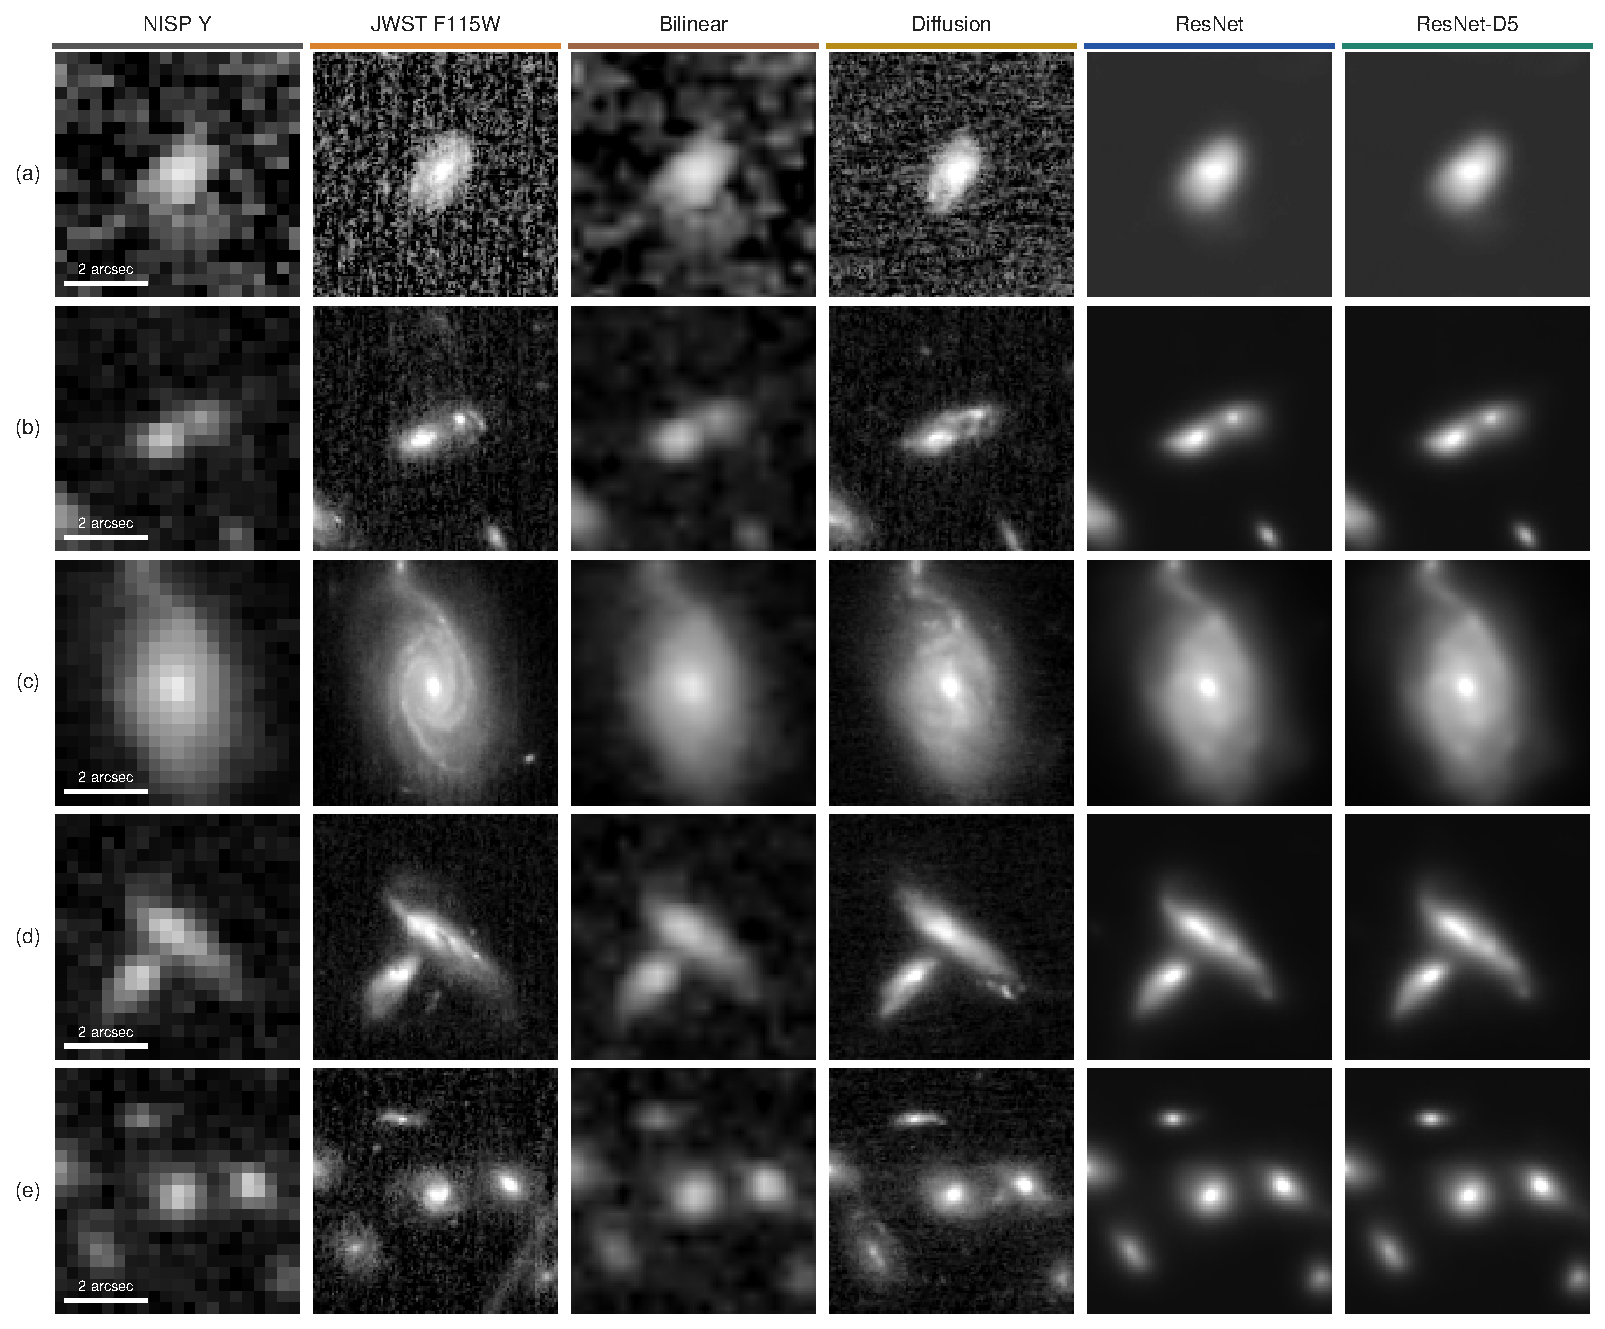
\includegraphics[width=\textwidth]{figs/galaxy_examples_v08.pdf}
    \caption{Observed images and reconstructions for five selected validation fields: (a) a modest isolated galaxy, (b) a close projected pair, (c) a face-on disk, (d) overlapping extended sources, and (e) a crowded field with multiple neighbours.
    Columns show, from left to right, native \Euclid\ NISP $Y$, the JWST F115W reference, bilinear interpolation of NISP, and diffusion, ResNet, and ResNet-D5 reconstructions; ResNet-D5 denotes the direct-$5\times$ residual variant.
    All fields are observational cutouts, with no injected sources.
    Each row spans approximately $6.3$ arcsec and uses the same asinh intensity stretch in physical surface-brightness units across all columns; scale bars indicate $2$ arcsec.
    Bilinear interpolation retains the NISP band and instrumental response.
    Reconstructions use the validation-selected checkpoints at epoch 35 for diffusion and epoch 49 for both residual models; diffusion shows one fixed-seed realization with 50 sampling steps.
    The original examples were selected from observed images, and this arrangement combines an isolated source with fields containing multiple sources.
    The selection is illustrative rather than statistically representative, and projected neighbours need not be physically associated.}
    \label{fig:galaxy_examples}
\end{figure*}

Figure~\ref{fig:galaxy_examples} compares the three models on the same observed fields, from an isolated galaxy to close pairs and a crowded field.
The shared display scale within each row allows the reconstructions to be compared directly with the input and reference images.
These selected examples illustrate differences in source separation and recovered morphology; they do not by themselves establish a population-level ranking or calibrated shape recovery.

\subsection{Reconstruction accuracy and spatial structure}
\label{sc:reconstruction_results}

\begin{figure*}[t]
    \centering
    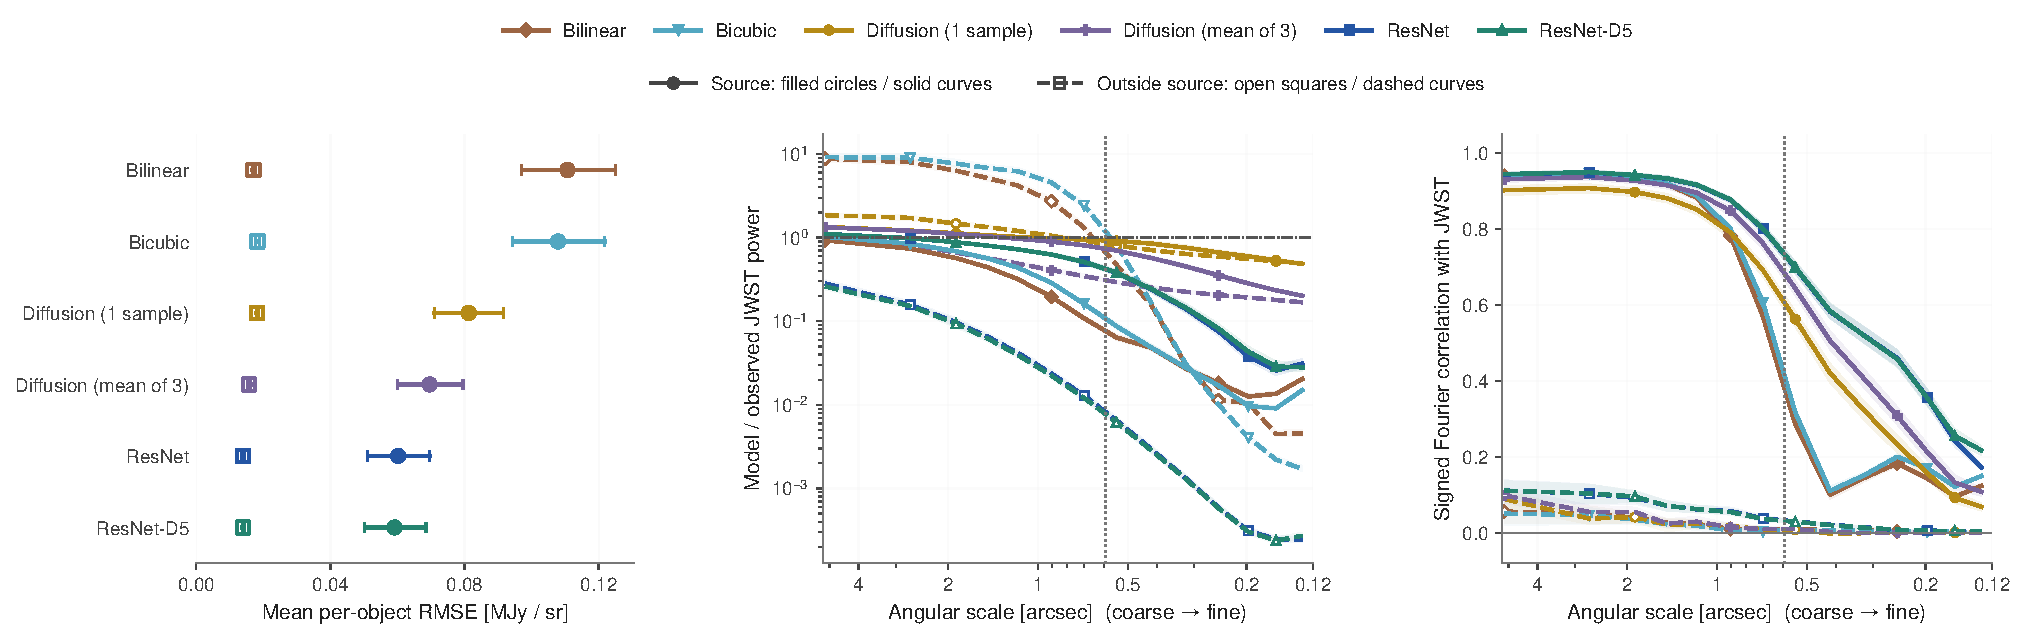
\includegraphics[width=\textwidth]{figs/model_comparison_v07.pdf}
    \caption{Reconstruction accuracy and spatial structure in reference-defined source and outside-source regions of the validation sample.
    Left: mean per-object RMSE against JWST F115W in signed, background-subtracted surface brightness for all 2118 objects, using common valid pixels in the central $105\times105$ target-pixel field.
    Filled circles indicate source pixels and open squares outside-source pixels; the same two-sigma JWST detection masks, including neighbours, are used for every method (Sect.~\ref{sc:regional_structure}).
    Middle: geometric mean model/reference power ratio. Right: mean signed annular Fourier correlation.
    Solid curves use sources in 1363 completely valid cutouts; dashed curves use outside-source pixels in the 1356 with sufficient window area.
    Each model and reference use identical windows, combining a three-pixel boundary taper and an outer Tukey window, after removal of each image's own weighted mean.
    Whiskers and shaded bands are 95\% intervals from 2000 paired spatial-block resamples over 18 blocks; they do not include training-seed variation.
    Colours identify methods; diffusion uses one fixed realization or the linear mean of three realizations.
    Checkpoints match Fig.~\ref{fig:galaxy_examples}: epoch 49 for ResNet and ResNet-D5, and epoch 35 for diffusion with 50 generation steps.
    The originally selected ResNet is retained; reproducibility and model-choice checks are summarized in Sect.~\ref{sc:resnet_selection}.
    The dotted vertical line marks the NISP pixel Nyquist wavelength, approximately $0\farcs593$, rather than an effective image resolution.
    Observed reference power includes noise; no noise subtraction, PSF correction, or window deconvolution is applied, and greater power agreement alone does not establish faithful recovery of individual features.}
    \label{fig:pixel_comp}
\end{figure*}

Figure~\ref{fig:pixel_comp} compares all methods on the same regional pixel support and separates reconstruction error from the amount and alignment of spatial variation.
Mean source RMSE is $0.06017$ and $0.05915$ MJy\,sr$^{-1}$ for ResNet and ResNet-D5, respectively, compared with $0.08123$ for a single diffusion realization, $0.06962$ for the mean of three diffusion realizations, and $0.11068$ for bilinear interpolation.
Outside-source RMSE is approximately $0.01396$ MJy\,sr$^{-1}$ for both residual models, compared with $0.01815$ for single diffusion and $0.01572$ for its mean image.
These regional averages describe the observed reference, including its noise and the NISP--F115W band difference.

The spectral panels show a complementary trade-off.
At wavelengths of 6--15 target pixels, the source power ratio is approximately 0.912 for single diffusion and 0.417 for ResNet, whereas the signed correlation is 0.604 and 0.737, respectively.
Diffusion retains more observed small-scale power, while the residual prediction has stronger agreement with the reference under the phase-sensitive correlation statistic.
Averaging diffusion realizations reduces power and increases correlation in this band.
The residual models nevertheless suppress substantial observed fine-scale power, so neither lower image error nor higher correlation should be interpreted as complete recovery of the JWST morphology.

\subsection{ResNet reproducibility and model choice}
\label{sc:resnet_selection}

Three independent 50-epoch ResNet training runs yield source RMSE values of $0.06007$--$0.06017$ MJy\,sr$^{-1}$ and outside-source values of $0.01393$--$0.01396$ MJy\,sr$^{-1}$ at their selected checkpoints.
The between-seed sample standard deviation of source RMSE is 0.09\% of its mean, distinct from the spatial-block uncertainty for any one trained model.
This supports reproducibility under the fixed recipe and data split, rather than robustness across surveys or training configurations.

The selected original-loss continuation reduces source RMSE by 1.21\% and outside-source RMSE by 0.09\% relative to the parent.
Equal source/outside-source weighting reduces source RMSE by 2.19\% but increases outside-source RMSE by 2.40\%, with no clear reduction in fixed or adaptive observed-shape RMSE on matched successful objects.
The PSF-aware continuations give only small additional reductions in source RMSE relative to the original-loss control: 0.12\% with PSF and noise inputs and 0.16\% when the inverse-filter feature is included.
The 95\% paired spatial-block intervals on both differences include zero.
The PSF/noise variant reduces fixed-weight shape RMSE by 0.98\% relative to the control, with a paired interval excluding zero, but neither variant clearly improves adaptive shapes.
These shape comparisons use 1627 common galaxies for fixed moments and 1700 for adaptive moments, matched across the selected and final checkpoints; their absolute errors are therefore not directly comparable with Fig.~\ref{fig:ellipticity_comp}.
The fixed visual examples remain very similar, and the fine-scale spatial correlation shows no clear additional gain over the control.
The experiment is limited to a warm start from one parent model and the small range of available stack PSFs, so it does not establish the performance of PSF-aware architectures more generally.

Together, these checks support retaining the original epoch-49 ResNet.
ResNet-D5 has slightly lower source RMSE and comparable observed-shape performance, while the original model has the additional evidence from three independent training seeds.
We use the original as the main model and retain D5 as a comparator, with the same 50-epoch budget for the primary architecture comparison.
This choice reflects the combined image and shape evidence rather than a claim that one network is best on every metric.

\subsection{Shape preservation}
\label{sc:shape_preservation}

\begin{figure*}[t]
    \centering
    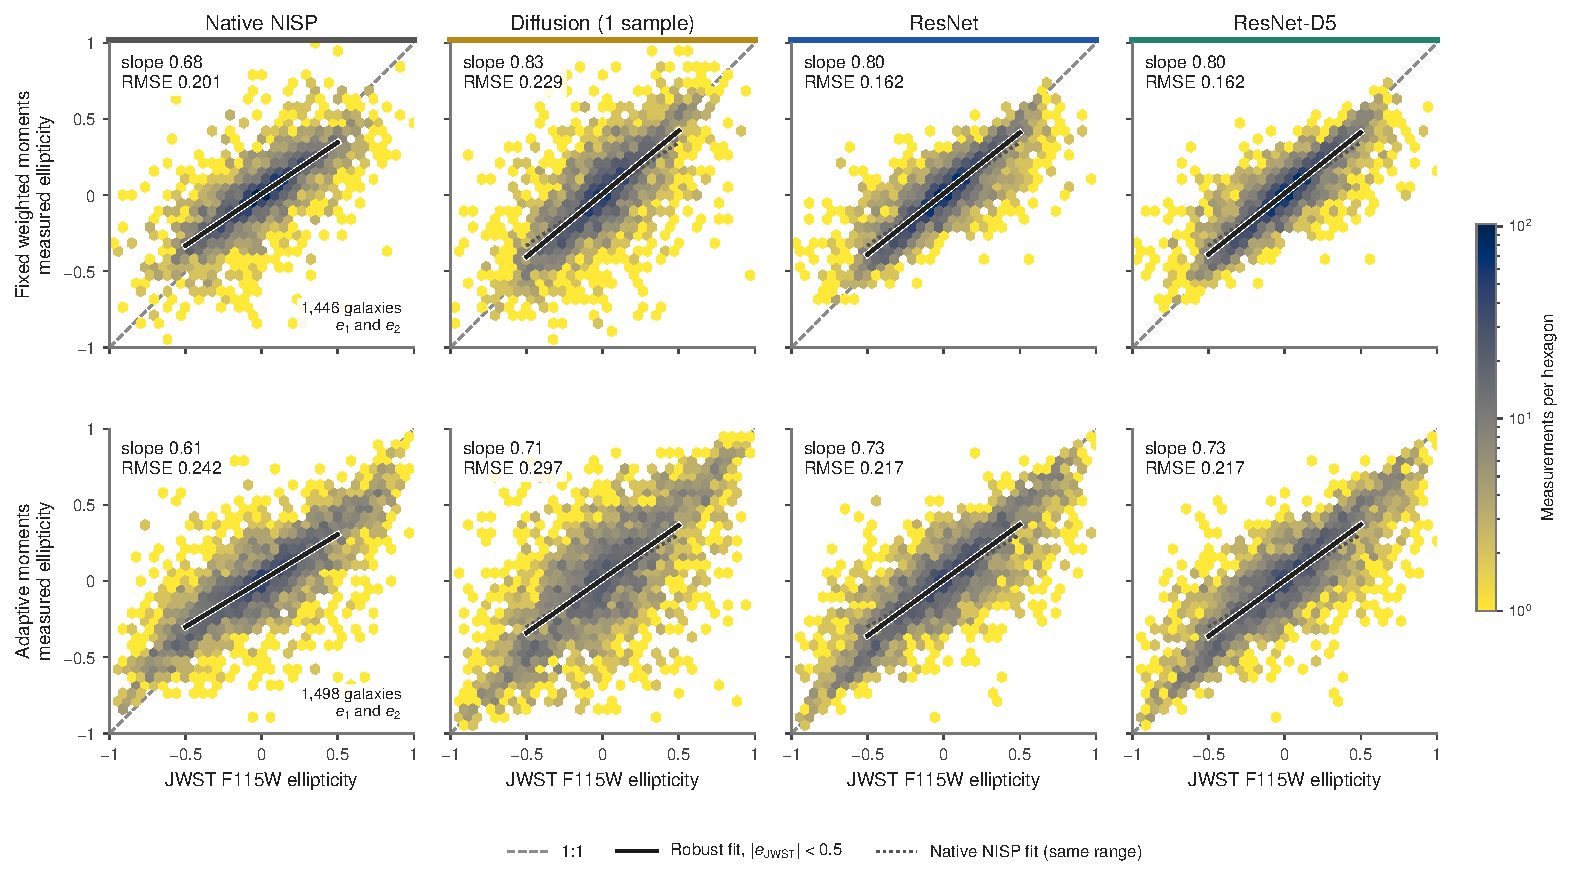
\includegraphics[width=\textwidth]{figs/shape_hexbin_v06.pdf}
    \caption{Observed ellipticity measured on native NISP, a single diffusion realization, ResNet, and ResNet-D5 (columns) against the same measurement on JWST F115W, using fixed weighted moments (top) and adaptive moments (bottom).
    Hexagonal bins share the logarithmic count scale shown by the colour bar; coloured header rules identify the methods; both components $e_1$ and $e_2$ enter for every galaxy in each estimator's common successful sample, 1446 galaxies for fixed moments and 1498 for adaptive moments, out of 2118 attempted validation fields.
    The dashed line is the 1:1 relation.
    The solid line is a Theil--Sen fit of measured against JWST ellipticity over galaxies with $|e_{\mathrm{JWST}}|<0.5$, drawn over that range; the dotted line in the model panels repeats the native-NISP fit.
    Each panel lists this slope and the full-sample RMSE about the 1:1 line, combining both components as $\sqrt{\langle(\Delta e_1^2+\Delta e_2^2)/2\rangle}$.
    Slope intervals and paired spatial-block intervals on the RMSE reduction are given in Sect.~\ref{sc:shape_preservation}.
    Native NISP is measured on its own pixel grid with the same angular weight and aperture; each model is measured on the $5\times$ target grid.
    Checkpoints match Fig.~\ref{fig:pixel_comp}.
    These are observed cross-band shapes that include instrumental PSF and pixel-sampling differences; they are not PSF-corrected morphologies or calibrated shear estimates.}
    \label{fig:ellipticity_comp}
\end{figure*}

Figure~\ref{fig:ellipticity_comp} compares the ellipticity of each reconstruction with the observed JWST ellipticity of the same galaxy, with native NISP as the reference point.
For fixed weighted moments, the core slope rises from 0.68 (95\% interval 0.66--0.70) for native NISP to 0.80 (0.77--0.83) for ResNet and ResNet-D5, and the RMSE about the 1:1 line falls from 0.201 to 0.162, a reduction of 19.3\% (16.6--21.9\%) from 2000 paired spatial-block resamples.
For adaptive moments the corresponding slopes are 0.61 (0.58--0.64) and 0.73 (0.71--0.75), with RMSE falling from 0.242 to 0.217, a reduction of 10.6\% (7.3--13.2\%).
A single diffusion realization also steepens the slope, to 0.83 and 0.71, but widens the distribution, so its RMSE exceeds native NISP by 13.8\% and 22.4\% for the two estimators.
The native-NISP core is itself narrow; the residual-model gain comes from the steeper relation and from fewer large errors rather than from a narrower core.

\subsection{Sensitivity to measurement choices}
\label{sc:robustness_results}

The original ResNet retains lower observed-shape RMSE than native NISP in all 21 measurement scenarios.
On the 1098 galaxies measurable in every scenario, the reduction ranges from 8.2\% to 25.0\%, with positive lower bounds for each marginal 95\% spatial-block interval.
The scenarios share galaxies and perturbations, so these intervals do not represent independent confirmations.
Background offsets produce the largest change: subtracting 0.1 outer-region RMS from the reconstruction reduces its measurement successes from 2045 to 1759 out of 2118 attempted objects, while the RMSE reduction on the common 1098-object sample falls from 19.0\% to 8.2\%.
The direction of improvement is thus stable under the tested choices, but its size and the number of usable measurements depend on the estimator and background treatment.

\subsection{Shape recovery versus input signal-to-noise}
\label{sc:shape_snr}

\begin{figure*}[t]
    \centering
    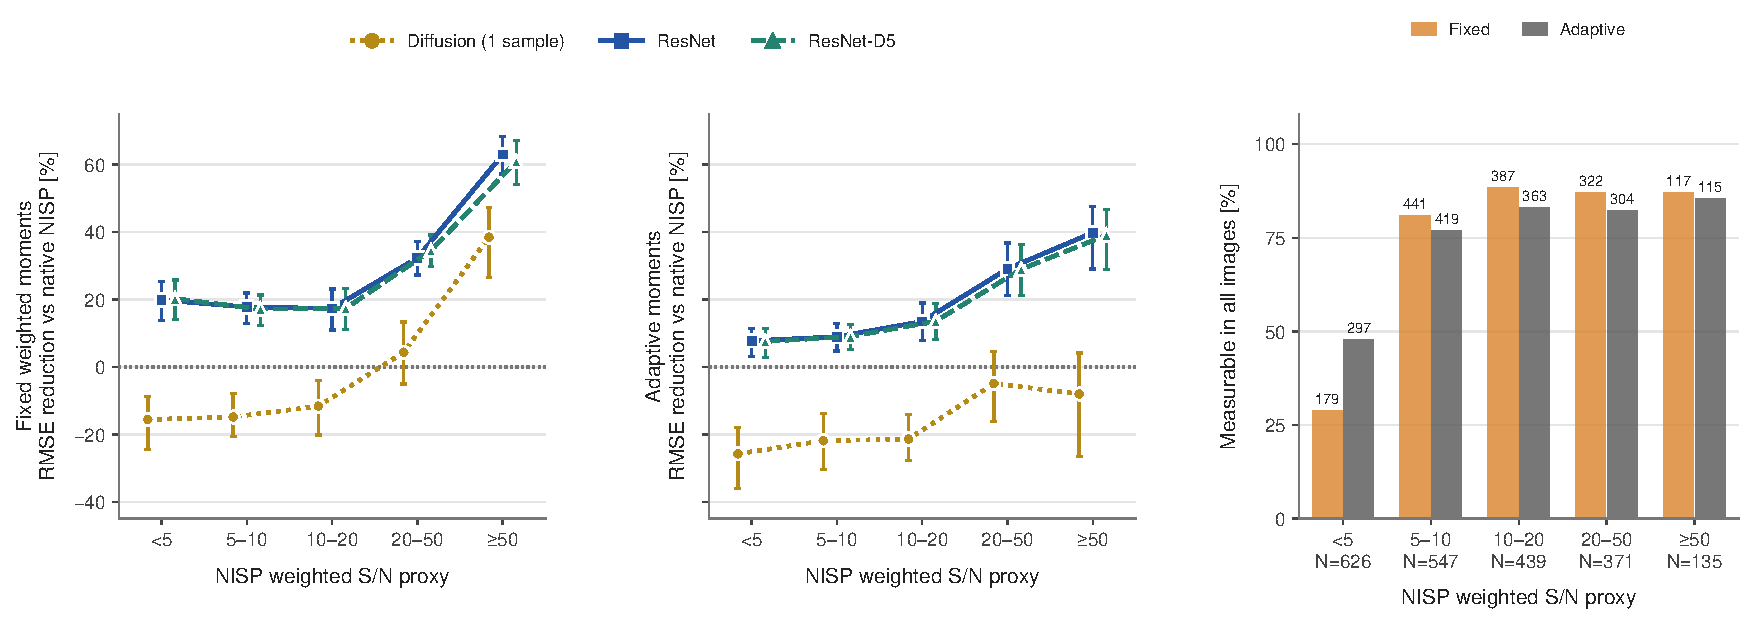
\includegraphics[width=\textwidth]{figs/shape_dependence_v04.pdf}
    \caption{Observed-shape recovery versus input NISP weighted S/N.
    Left and middle: percentage reduction in ellipticity-component RMSE relative to native NISP, for fixed weighted and adaptive moments, respectively; positive values indicate lower error against observed JWST F115W.
    Ochre circles, cobalt squares, and green triangles denote a single diffusion realization, ResNet, and ResNet-D5.
    Each estimator/bin uses the same galaxies measurable in JWST, native NISP, and all six reconstruction/interpolation methods.
    Points are horizontally offset for visibility; the bins are categorical and connecting lines guide the eye.
    Whiskers show conditional 95\% intervals from 2000 paired spatial-block resamples, not simultaneous intervals for a trend.
    Right: common measurement coverage among all attempted fields, with fixed moments in solid orange and adaptive moments in hatched charcoal.
    Numbers above bars are common successes; $N$ below each bin gives the attempted count.
    Totals are 1446 fixed-moment and 1498 adaptive-moment successes out of 2118 validation fields.
    The S/N proxy neglects correlated noise, and fixed and adaptive moments have different successful samples.
    These observed cross-band comparisons include PSF and pixel-sampling differences and do not measure calibrated shear.}
    \label{fig:shape_snr}
\end{figure*}

Figure~\ref{fig:shape_snr} shows positive native-relative RMSE reductions for both residual networks in every input-S/N bin under both estimators.
For ResNet, the reduction is 19.9\% (13.8--25.3\%) for fixed moments and 7.8\% (3.2--11.4\%) for adaptive moments at S/N below 5, rising to 63.0\% (57.3--68.3\%) and 39.8\% (29.1--47.6\%), respectively, at S/N at least 50.
ResNet-D5 follows a similar dependence.
A single diffusion realization has larger errors than native NISP at S/N below 20 under both estimators.
Its highest-S/N fixed-moment reduction is 38.5\% (26.6--47.2\%), while its adaptive-moment interval includes zero.

The low-S/N comparison represents a selected measurable subset: only 179/626 fields (28.6\%) enter the fixed-moment comparison and 297/626 (47.4\%) enter the adaptive comparison in the lowest bin.
The coverage is the intersection across all images, not an individual model's success rate.
Repeating the comparison on the common population shared by both estimators retains positive ResNet gains in every bin.
The larger high-S/N gains are descriptive: S/N and the native baseline share input pixels, while galaxy size, brightness, crowding, and redshift can also vary between bins.
These results do not imply that all faint sources become useful shape measurements or isolate a causal effect of changing S/N.

\subsection{Response to applied shear}
\label{sc:shear_response_results}

\begin{figure*}[t]
    \centering
    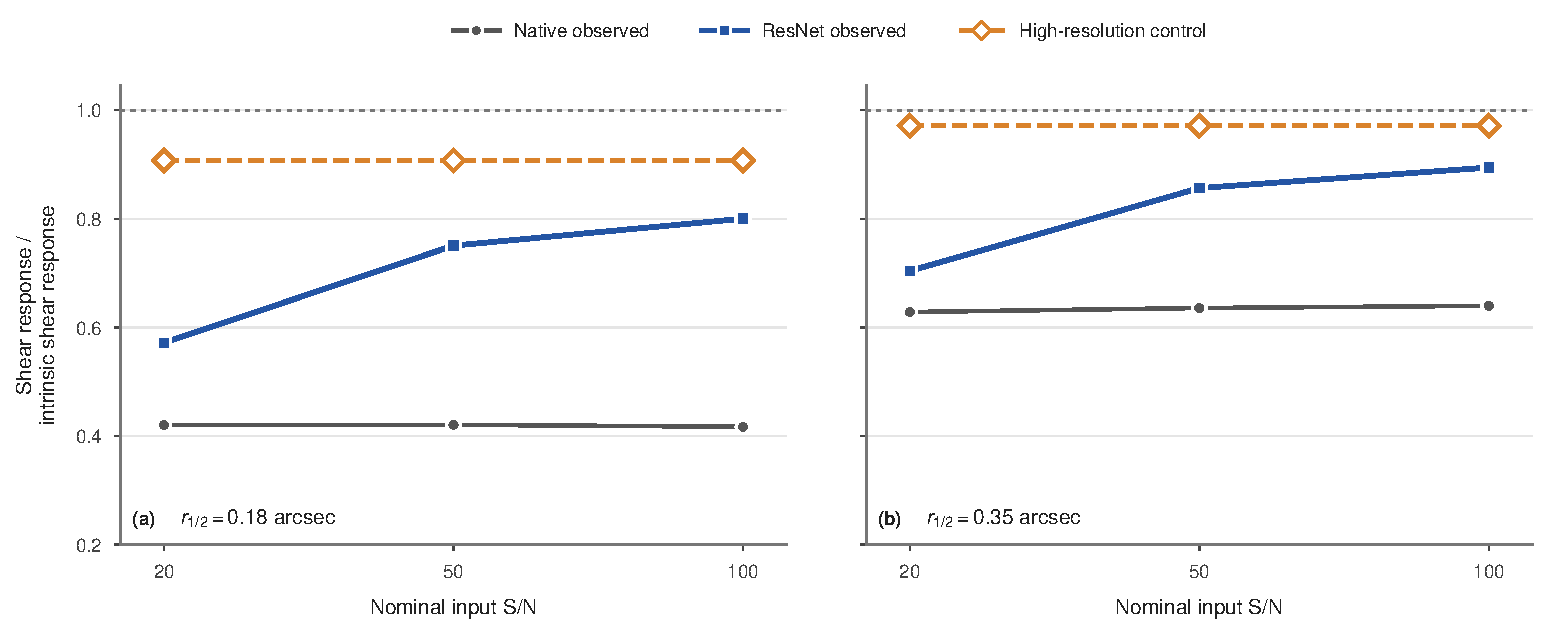
\includegraphics[width=\textwidth]{figs/shear_response_v06.pdf}
    \caption{Controlled shear response of observed adaptive shapes using the four supplied NISP effective PSFs.
    Panels (a) and (b) show exponential galaxies with intrinsic half-light radii $0\farcs18$ and $0\farcs35$.
    Charcoal circles, cobalt squares, and orange open diamonds denote native NISP, the original ResNet, and a noiseless high-resolution control.
    The vertical axis is $\mathrm{tr}(R)/\mathrm{tr}(R_{\rm intrinsic})$; the dotted line marks the intrinsic response.
    Each point equally averages the four per-PSF ratios on identical objects successful across all PSFs, methods, and five shear branches.
    Each noisy cell attempts eight orientations and four noise realizations per orientation; the common sample is 31/32 at radius $0\farcs18$ and S/N 20, and 32/32 elsewhere in the displayed grid.
    The same noise is reused across shear branches and PSFs.
    S/N positions are categorical and connecting lines guide the eye; these are point estimates without uncertainty intervals.
    The high-resolution control uses a Gaussian PSF of FWHM $0\farcs08$, not a validated JWST PSF.
    The two radii were selected for their larger gains in the earlier Gaussian-PSF pilot; the full new grid also includes radius $0\farcs65$ and noiseless native inputs.
    No PSF correction is applied to these shapes, and the responses do not establish calibrated weak-lensing accuracy.}
    \label{fig:shear_response}
\end{figure*}

The controlled experiment completes all 48 PSF/size/S/N cells, corresponding to 6240 sheared native inputs.
Figure~\ref{fig:shear_response} shows higher normalized shear response for ResNet than for native NISP in all six displayed size/S/N combinations.
At S/N 100, the ratios are 0.800 and 0.894 for ResNet at radii $0\farcs18$ and $0\farcs35$, compared with 0.417 and 0.640 for native NISP; the high-resolution control gives 0.907 and 0.971.
ResNet therefore retains more sensitivity to the applied distortion in these cases, but remains below both the intrinsic and high-resolution-control responses.

The improvement is not uniform across the full grid.
At radius $0\farcs65$ and S/N 20, the ResNet response is 0.715, below the native value of 0.774; at S/N 50 and 100, the corresponding ResNet/native ratios are 0.854/0.810 and 0.921/0.819.
Noiseless-input ResNet responses are 0.806, 0.924, and 0.951 at radii $0\farcs18$, $0\farcs35$, and $0\farcs65$.
The two displayed radii were chosen during the preceding Gaussian-PSF pilot, before the supplied-PSF rerun, so they should not be interpreted as an unbiased size selection.
Finite PSF stamps and header geometry, exponential profiles at a fixed pixel phase, independent pixel noise, and conditioning on successful measurements limit the experiment's realism.
It does not include realistic morphology and blending distributions, correlated stack noise, chromatic effects, or the full selection response required for shear calibration.

\section{\label{sc:discussion}Discussion}

The residual models achieve lower image errors and stronger spatial correlation with the observed JWST reference, while diffusion retains more small-scale power (Fig.~\ref{fig:pixel_comp}).
Together, these measurements explain why apparent sharpness alone is an incomplete measure of reconstruction quality: a prediction can contain fine-scale variation without placing it where it appears in the reference.
The residual reconstructions provide more accurate images under the tested metrics, although their reduced power shows that some observed detail is smoothed away.
The comparison includes noise, different instrumental responses, and the difference between the \YE\ and F115W passbands.

The repeated training runs and targeted follow-up experiments provide a practical basis for choosing the original ResNet.
Its reconstruction errors are consistent across three seeds, and neither the modified loss nor the PSF-aware inputs produce a clear improvement across image and shape measures beyond the extra-training control.
The small fixed-weight shape gain from PSF/noise conditioning is nevertheless worth investigating with more varied PSFs and independent training runs.
The present experiments constrain the benefit of these particular modifications; they leave room for better objectives, architectures, and training data.

The shape comparisons and controlled simulations show two useful consequences of the reconstruction.
Observed ellipticities agree more closely with JWST, and compact simulated galaxies retain more sensitivity to an applied shear after passing through ResNet.
These gains depend on the conditions: low-S/N shape comparisons include only a subset of attempted galaxies, and the largest simulated galaxies at low S/N provide a counterexample to uniform response improvement.
The cross-band ellipticity slopes describe agreement between observed images and cannot be interpreted as multiplicative shear calibration factors.
For cosmological use, the remaining response deficit must be addressed with a validated treatment of measurement and selection response across realistic morphologies, sizes, noise, blends, and spatially varying PSFs.
The required control of multiplicative shear bias, at approximately $10^{-3}$ for \Euclid\ \citep{Cropper2013}, remains a separate validation target.

The scope of the training sample also matters for the proposed application.
Our galaxies lie in one COSMOS field and satisfy F814W $<25$ and $z_{\rm phot}<3$.
The results therefore do not yet demonstrate performance on the optically fainter population that motivates extending shape measurements into the near-infrared.
The observed-image comparisons use validation data that also informed model and measurement choices.
An independent evaluation on the 2876 reserved test galaxies is still needed to assess the fixed procedure, followed by tests across fields and galaxy populations.

The image and shape improvements also motivate applications with different requirements from cosmic shear, including morphology, deblending, and strong-lens searches.
Residual networks have already been used to identify strong-lens candidates in the DESI Legacy Imaging Surveys \citep{Huang_et_al_2021}, and learned image reconstruction has been explored for deblending and sharpening \citep{superres_1, Reiman_Gohre_2019, Arcelin2021, Hemmati2022, superres_2}.
Testing whether NISP reconstruction improves such tasks would require their own labelled samples and performance measures.
Further development should also quantify residual astrometric offsets and the effective PSFs of the input, target, and reconstructed images, since these determine how image differences translate into morphological errors.

\section{Conclusions}
\label{sc:conclusions}

Learned reconstruction improves the fidelity of NISP imaging to the observed JWST F115W reference in this validation sample.
Residual networks give lower image errors and stronger spatial correlation than the tested diffusion model, while the original ResNet reduces observed ellipticity-component RMSE by approximately 19\% with fixed weighted moments and 11\% with adaptive moments on matched successful galaxies.
Independent training runs reproduce its image errors, and controlled simulations show increased shear response for compact galaxies under the tested PSFs and noise levels.
These results support ResNet as a promising starting point for extracting more structural information from NISP imaging.
Evaluation on the reserved test sample and realistic simulations of instrumental, noise, and selection effects will establish how far these gains can support morphological and weak-lensing applications.

\section*{Data and code availability}

The \Euclid\ images are available through Quick Release Q1 \citep{Q1cite}, and the JWST mosaics through the COSMOS-Web public data release\footnote{\url{https://cosmos2025.iap.fr/}}.
The sample selection uses the public COSMOS2020 Classic catalogue \citep{cosmos2020_classic}.
The trained model weights and code for preparing the paired sample, training the networks, and reproducing the analyses and figures will be released publicly with publication.
% Add the persistent archive link when the code and model release is deposited.

%
% Add the acknowledgement using the achnowledgements environment.
% Do not use \acknowledgement{....} as this affects the formatting
% of the references.
%

\begin{acknowledgements}
\AckQone
\AckEC  
\end{acknowledgements}

%
% Here comes the reference list, generated via bibtex from
% your bibfile my.bib and Euclid.bib. Please make sure that
% the same paper is not referenced twice, one from your my.bib
% file, and once from Euclid.bib.
%

\bibliography{Euclid, mybib}
%
% You can have different .bib files here, e.g.
% \bibliography{Euclid,myown}, but please use the bibentries
% in Euclid.bib for all EC publications to ensure that these
% references are up-to-date and in correct format.
%


\label{LastPage}
\end{document}
